\documentclass[conference]{IEEEtran}
\IEEEoverridecommandlockouts

\usepackage{graphicx}
\usepackage{amsmath,amssymb,amsfonts,amsthm}
\DeclareMathOperator{\lcm}{lcm}
\usepackage{paralist}
\usepackage{color}
\usepackage[hidelinks]{hyperref}
\usepackage{xspace}
\usepackage{algorithm}
\usepackage{algorithmicx}
\usepackage{todonotes}
\usepackage{verbatim}

\usepackage{array}
\newcolumntype{L}[1]{>{\raggedright\let\newline\\\arraybackslash\hspace{0pt}}m{#1}}
\newcolumntype{C}[1]{>{\centering\let\newline\\\arraybackslash\hspace{0pt}}m{#1}}
\newcolumntype{R}[1]{>{\raggedleft\let\newline\\\arraybackslash\hspace{0pt}}m{#1}}

\usepackage{gnuplot-lua-tikz}

\newtheorem{example}{Example}
\newtheorem{theorem}{Theorem}

\newcommand*{\email}[1]{\href{mailto:#1}{\nolinkurl{#1}} }
\newcommand{\ie}[0]{\emph{i.e.}\xspace}
\newcommand{\eg}[0]{\emph{e.g.}\xspace}

\newcommand{\muind}{\mu_{\text{ind}}}
\newcommand{\bandtotal}{\beta_{\text{tot}}}
\newcommand{\bandavail}{\beta_{\text{avail}}}
\newcommand{\appset}{{\mathcal A}}
\newcommand{\nbnodesplat}{{\mathcal N}}
\newcommand{\nbapps}{|{\mathcal A}|}
\newcommand{\app}[1]{A_{#1}}
\newcommand{\application}[2]{a_{#1}^{#2}}
\newcommand{\nbapp}[1]{n_{#1}}
\newcommand{\nbnodes}[1]{q_{#1}}
\newcommand{\period}[1]{P_{#1}}
\newcommand{\ckpt}[1]{C_{#1}}
\newcommand{\reco}[1]{R_{#1}}
\newcommand{\size}[1]{\mathit{size}_{#1}}
\newcommand{\wasteapp}[1]{W_{#1}}
\newcommand{\wap}[1]{W_{#1}}
\newcommand{\wapp}[2]{W_{#1}(#2)}
\newcommand{\mtbfplat}{\mu}
\newcommand{\wasteplat}{W}
\newcommand{\ioconstraint}{F}
\newcommand{\lastckpt}[2]{L_{#1}^{#2}}
\newcommand{\wastefct}[2]{W_{#1}(#2)}
\newcommand{\pool}{{\mathcal P}}
\newcommand{\risk}{{\textsc Risk}}
%\newcommand{\todo}[1]{\textit{TBD: [#1]}}
\newcommand{\dca}[1]{\todo[inline]{DCA: #1}}

\newcommand{\IOcat}{\textsc{IO-Candidate}\xspace}
\newcommand{\Ckptcat}{\textsc{Ckpt-Candidate}\xspace}
\newcommand{\Catiocat}{\mathcal{C}_{IO}\xspace}
\newcommand{\Catckptcat}{\mathcal{C}_{Ckpt}\xspace}

\newcommand{\nocoop}{\emph{Oblivious}\xspace}
\newcommand{\fifoblock}{\emph{Ordered}\xspace}
\newcommand{\fifononblock}{\emph{Ordered-NB}\xspace}
\newcommand{\leastwaste}{\emph{Least-Waste}\xspace}

\def\propfixedlong{\nocoop, Fixed checkpointing period (1h)\xspace}
\def\propfixed{\nocoop-Fixed\xspace}
\def\propdalylong{\nocoop, Daly checkpointing period\xspace}
\def\propdaly{\nocoop-Daly\xspace}

\def\bfifofixedlong{\fifoblock, Fixed checkpointing period (1h)\xspace}
\def\bfifofixed{\fifoblock-Fixed\xspace}
\def\bfifodalylong{\fifoblock, Daly checkpointing period\xspace}
\def\bfifodaly{\fifoblock-Daly\xspace}

\def\fifofixedlong{\fifononblock, Fixed checkpointing period (1)\xspace}
\def\fifofixed{\fifononblock-Fixed\xspace}
\def\fifodalylong{\fifononblock, Daly checkpointing period\xspace}
\def\fifodaly{\fifononblock-Daly\xspace}

\def\cooperativelong{Cooperative \leastwaste Scheduling of Checkpoints and I/O\xspace}
\def\cooperative{\leastwaste\xspace}



\title{Optimal Cooperative Checkpointing for Shared High-Performance Computing Platforms
\thanks{NSF Award \#1564133 Toward Extreme Scale Fault-Tolerance: Exploration Methods, Comparative Studies and Decision Processes.}
}

\author{
\IEEEauthorblockN{Thomas Herault\IEEEauthorrefmark{1},
Yves Robert\IEEEauthorrefmark{2}\IEEEauthorrefmark{1},
Aurelien Bouteiller\IEEEauthorrefmark{1},
Dorian Arnold\IEEEauthorrefmark{3},\\
Kurt B.~Ferreira\IEEEauthorrefmark{4},
George Bosilca\IEEEauthorrefmark{1},
Jack Dongarra\IEEEauthorrefmark{1}}
\IEEEauthorblockA{\IEEEauthorrefmark{1}Innovative Computing Lab.
The University of Tennessee,Knoxville, TN, USA\\
\IEEEauthorrefmark{2}ENS Lyon, Lyon, France\\
\IEEEauthorrefmark{3}Emory University, Atlanta, GA, USA\\
\IEEEauthorrefmark{4}Center for Computing Research, Sandia National Laboratory\thanks{
Sandia National Laboratories is a multimission laboratory managed and operated
by National Technology and Engineering Solutions of Sandia, LLC., a wholly owned
subsidiary of Honeywell International, Inc., for the U.S. Department of Energy’s
National Nuclear Security Administration under contract DE-NA0003525.}
}
}

\begin{document}

\maketitle

\begin{abstract}
% Primary: George & Dorian
  In high-performance computing environments, input/output (I/O) from various
sources often contend for scare available bandwidth. Adding to these I/O
operations inherent to the failure-free execution of these applications, I/O
from checkpoint/restart (CR) operations used to ensure progress in the presence
of failures,  places an additional burden as it increases I/O contention which
leads to degraded performance.
%  aggravates the problem. Without careful consideration, contending I/O from
%  independently operating sources will lead to significant performance
%  degradation.  especially for capacity I/O loads such as the I/O from
%  checkpoint/restart (CR) services used to protect these computations from
%  platform faults.  For example, I/O from concurrently running applications
%  can contend with each other as well as with other I/O loads, such as the I/O
%  from checkpoint/restart (CR) services used to protect these computations
%  from platform faults.
  In this work, we consider a cooperative scheduling policy that optimizes the
overall performance of concurrently executing CR-based applications which share
valuable I/O resources.  First, we provide a theoretical model and derive a set
of necessary constraints needed to minimize the global \emph{waste} on the
platform.
%  the scientific throughput of these platforms. Using this cooperative policy,
%  application checkpoints are cooperatively orchestrated to prevent congestion
%  and to minimize the global waste.
  Our results demonstrate that the optimal checkpoint interval as defined by
Young/Daly, while providing a sensible metric for a single application, is not
sufficient to optimally address resource contention at the platform scale.  We
therefore show that combining optimal checkpointing periods with I/O scheduling
strategies can provide a significant improvement on the overall application
performance, thereby maximizing platform throughput.
%   sequentially, with a dynamic, priority-dependent frequency dictated by the
%   scheduler. When enough I/O bandwidth is available, each application
%   checkpoints with its optimal period. However, when I/O bandwidth is scarce,
%   our scheduling algorithm provides an optimal checkpoint process that
%   maximizes platform throughput. Our results show ...
Overall, these results provide critical analysis and direct guidance on checkpointing
large-scale workloads in the presence of competing I/O while minimizing the impact
on application performance.

\end{abstract}

% !TEX root =  ipdps18.tex

\section{Introduction}
\label{sec:intro}
% Primary: George & Dorian

%space sharing but not quite
\emph{Space-sharing} high-performance computing (HPC) platforms for the
concurrent execution of multiple parallel applications is the prevalent usage
pattern in today's HPC centers.  In fact, space-sharing in this fashion is more
common than \emph{capability} workloads that span the entire
platform~\cite{Weidner2016}. Furthermore, while computational nodes are
dedicated to a particular application instance, the interconnect links and
storage partition are typically shared amongst application instances. Therefore,
without careful consideration, network and storage contention can reduce
individual application and overall system performance \todo{kbf: CITE "There goes the
neighborhood"?}.

On these platforms, checkpoint/restart (CR) is the most common strategy
employed to protect applications from underlying faults and failures.
Generally, CR periodically outputs snapshots (i.e. checkpoints) of its global,
distributed state to some stable storage device. When an application failure
occurs, the last stored checkpoint is retrieved and used to restart the
application.  Typically, concurrently executing applications independently
decide when to take their own checkpoints.

There are two widely-used approaches to determine when an application should
\emph{commit} a checkpoint: (i)~using a fixed checkpoint period (typically one
or a few hours) for each application; and (ii)~using platform and
application-specific metrics to determine its optimal checkpoint period. In the
second approach, the well-known Young/Daly formula~\cite{young74,daly04} yields
an application optimal checkpoint period, $\sqrt{2 \mu C}$ seconds, where $C$
is the time to commit a checkpoint and $\mu$ the application Mean Time Between
Failures (MTBF) of the platform.  In most cases, $\mu = \frac{\muind}{q}$,
where $q$ is the number of processors enrolled by the application and $\muind$
is the MTBF of an individual processor~\cite{springer-monograph}. Therefore,
both $\mu$ and $C$ in the Young/Daly formula are application-dependent, and
optimal periods can be quite different over the application spectrum.

Independent CR of concurrent application instances can incur significant
resource wastage, because they lead to an inefficient usage of an already
scarce resource, namely available I/O bandwidth\todo{kbf: CITE R. Ross SOP
paper?}.  There are two major reasons for this:

\begin{enumerate}
        
\item \emph{Application-CR I/O contention}: On many systems, the I/O subsystem
does not have enough available usable bandwidth to meet the requirements of
the concurrent application workloads\todo{kbf: CITE R. Ross SOP paper?}. This
congestion is expected to worsen going forward with the emergence of many data
intensive workloads in HPC\todo{kbf: CITE}.  Let $\bandtotal$ be the total
filesystem I/O bandwidth.  Concurrently executing applications typically
perform regular (non-CR) I/O operations throughout their execution, so that
only a fraction $\bandavail$ of the total bandwidth remains available for
checkpoints.  This fraction may be insufficient, particularly when some
applications perform intensive non-checkpoint I/O and others may write very
large checkpoints.
  % $\bandtotal$ of a well-provisioned platform should allow for efficient CR
  % I/O activities.

\item \emph{CR-CR I/O contention}: Most importantly, there is a high
probability of overlapping CR activity amongst concurrent application
instances.  Consider the simple case where two applications of same size
checkpoint simultaneously a file of the same size. Each will be assigned half
the fraction $\bandavail$ to checkpoint, therefore the commits will take twice
as long. Such interferences can severely decrease application efficiency and
overall platform throughput (e.g., when the expected checkpoint commit time
used to compute the optimal checkpoint interval differs from the actual
checkpoint commit time)\todo{footnote?}.

\end{enumerate}

In this work, we develop and investigate a cooperative CR scheduling strategy
for concurrently executing HPC applications.  Our objective is to assess the
impact of such interferences and to design scheduling algorithms that optimize
I/O bandwidth availability for CR activity.  Using these cooperative
algorithms, applications checkpoint sequentially, with a dynamic,
priority-dependent frequency dictated by a cooperative scheduler.  When enough
I/O bandwidth is available, each application checkpoints with its optimal,
Young/Daly, period.  However, when I/O bandwidth is scarce, our scheduling
algorithm provides an optimal checkpoint period that maximizes overall platform
throughput. This cooperative checkpoint process is calculated such that there
is no I/O interference and minimal re-work to be done when failures occur.

Therefore, the main contributions of this paper are the following:

\begin{itemize}

\item Development of a model allowing for the quantification of
the I/O interference of checkpointing applications sharing a common underlying I/O
substrate.

\item Investigation of the costs of various I/O-aware scheduling
strategies through both steady-state analysis as well as detailed simulations.

\item A detailed survey of a number scheduling strategies: from oblivious
algorithms similar to  those currently deployed on many large-scale platforms,
to ones which exploit application knowledge in an effort to  minimize the total
system waste by scheduling the application with the most critical I/O needs.

\end{itemize}

% - a model to predict the shared I/O impact on multiple applications scenarios
% - I/O scheduling algorithms for non-cooperative application scheduling
%   - non-cooperative I/O scheduling: apps are selected to fill the gaps based on processor count (traditional approach)
%   - blocking FIFO I/O scheduling: favor one of the I/O application
%   - non-blocking FIFO I/O scheduling: same as above but the cost of the queueing the app is now independent of the interference pattern
%   - least-waste algorithm: select the app that will minimize the system waste (I/O or C/R candidate)
% - steady state analysis
% - simulation
% - results

The rest of the paper is organized as follows. Our model is described in
\Cref{sec:model}, followed by a description of the various scheduling
strategies in \Cref{sec:algorithms}. \Cref{sec:lowerbound} presents a
theoretical analysis of the model under a steady-state scenario, and provides a
lower bound of the optimal platform waste. \Cref{sec:simulator} describes the
discrete event simulator used to quantitatively compare the different
scheduling strategies.  \Cref{sec:results} presents the results of the
simulation, providing guidance on the necessary I/O bandwidth for  current and
future systems. This work concludes with related works described in \Cref{sec:related},
followed by a summary and future directions outlined in \Cref{sec:conclusion}.

% - Section~\ref{sec:model} describe the scenario under investigation
% - Section~\ref{sec:algorithms} describe the different I/O scheduling
%   algorithms that we plan to analyze, including one that is highly related to
%   the default scheduling on most HPC platforms
% - Section~\ref{sec:lowerbound} describe a theoretical scenario that allow us
%   to derive the lower-bound
% - Section~\ref{sec:simulator} describe the simulator used to validate the
%   results
% - Section~\ref{sec:results} present the results
% - Section~\ref{sec:related} depicts the related work field
% - Section~\ref{sec:conclusion} conclude

% !TEX root =  ipdps18.tex

\section{Model}
\label{sec:model}
% Primary: Yves

%\todo[inline]{Question: how can we consider applications with finite time, initial
%  input and final output? Current idea is to distribute complete
%  volume of I/O over wall time, then take a single fake schedule that
%  assign resources to the apps following a distribution, and say 'it
%  shouldn't be far from finite apps being scheduled eagerly over
%  finite resource for a long time, in average'.}

\paragraph{Computational Platform Model}
In this work, we consider a shared platform that comprises a set of computational
nodes, storage resources in the form of a parallel file system (PFS), and a network
that interconnects the nodes as well as the storage resources. Applications are
scheduled on the platform by a job scheduler such that computational nodes are
space-shared (dedicated) amongst concurrent application instances. However, the I/O
subsystem is time-shared (contended) amongst the application instances, \ie multiple
applications performing I/O simultaneously can result in a per-application reduction
in commit speed. Without loss of generality, we consider a straightforward linear
interference model in which the global throughput remains constant and is evenly
shared among contending applications. (A more adversarial interference models could
be substituted.)

\paragraph{Application Workload Model}
Applications can vary in size (number of computational nodes), duration, memory
footprint and I/O requirements.  \emph{Application I/O} entails loading an input file
at startup, performing regular I/O operations during their main execution phase and
storing an output file at completion. Because applications are long-running
(typically, several hours or days) and the platform is failure-prone, applications
are protected using coordinated CR that incurs periodic \emph{CR I/O}.

To model these behavioral variations with minimal parameters, we make the following
simplifying assumptions (that we validate in the experimental section):
\begin{compactitem}
\item There is a large number of applications, but only a small number of application
  classes, \ie, sets of applications with similar sizes, durations, footprints and
  I/O requirements;
\item Other than initialization and finalization I/O, an application's regular
  (non-CR) I/O operations are evenly distributed over its makespan.
\item Job makespans are precisely known a priori. This allow us to ignore all other
  sources of job disturbance except C/R overheads.
\end{compactitem}
We used specific numbers and characteristics of application classes based on real
benchmark data, such as the APEX benchmark on the Cielo platform~\cite{apex2016}.  To
avoid the side effects induced by hundreds of completely identical application
instances, we use normal distributions for job durations with mean equal to original
APEX value and small (10\%) standard deviation.

\paragraph{Checkpoint Period and I/O Interference}

Both application computation and CR generate I/O requests, and both classes of I/O
activity are scheduled using the same algorithm (Section~\ref{sec:algorithms}). As
described above, steady-state application I/O is regular. However, CR I/O
periodicity, $P$, depends
upon the CR policy being used.  In our model, applications either checkpoint using an
application-defined periodicity or using Young and
Daly's~\cite{young74,daly04} optimal checkpoint period. The latter interval is
computed by, $T=\sqrt{2 C \mu}$, where $C$ is the duration of the checkpoint
transfer, and $\mu$ is the application mean time between failures (MTBF).
$\mu = \frac{\muind}{q}$, where $q$ is the number of processors enrolled by the
application and $\muind$ is the MTBF of an individual
processor~\cite{springer-monograph}.  The parameters in this formula are dependent
upon application features (checkpoint dataset size) and platform features (system
reliability and I/O bandwidth).

Traditionally, when an application, $\app{i}$, completes a checkpoint, its next
checkpoint is scheduled to happen in at least $\period{i}-\ckpt{i}$ (and the first
checkpoint is set at date $\period{i}$).  With potential CR I/O interference,
determining the appropriate checkpointing period can be challenging.
% The observed duration of checkpoints varies depending on how much interference
% happen, on average.
Additionally, I/O scheduling algorithms that try to mitigate I/O interference can
impose further CR I/O delays.  In other words, the traditional strategy of scheduling
subsequent checkpoints at $\period{i}-\ckpt{i}$ yields the desired checkpointing
period $\period{i}$ only in interference-free scenarios. CR I/O delays (induced by
interferences or scheduling delays) dilate the checkpoint duration to $C_{dilated}$,
and the effective period differs from the desired period by the difference
$C_{dilated}-\ckpt{i}$.  (In Section~\ref{sec:algorithms}, we discuss how each I/O
scheduling algorithm accommodates this discrepancy.)

%TODO: do we want to talk about that, if only to say we don't care?
%  {we may want to separate Input+recovery from output+checkpoint (bidirectional channels)}
%  {answer: we could but not sure it is 100\% independent; and it would complicate things without changing the story.}


\paragraph{Job Scheduling Model}
To evaluate the scheduling policies, we consider a finite segment, typically lasting
a small number of days, of a representative schedule where the number of application
instances (jobs) in each class remains approximately constant at every instant. Of
course, with different job execution times, we cannot enforce a fixed proportion of
each application class at every instant. However, we ensure the proper proportion is
enforced in average throughout the schedule execution. Similarly, we enforce that at
every instant during the finite segment, at least 98\% of the nodes are enrolled for
the execution. This allows us to compare actual (simulated) performance with the
theoretical performance of a co-scheduling policy that optimizes the steady-state I/O
behavior of the job portfolio, assuming that all processors are used. We shuffle and
simultaneously present all jobs to the scheduler, which uses a simple, greedy
first-fit algorithm.  We resubmit failed jobs with a new wall-time equal to the
fraction that remained when the last checkpoint was committed. Input I/O becomes
recovery I/O; output I/O is unmodified.

\paragraph{The Formal Model}
We consider a set $\appset$ of $\nbapps$ applications classes
$\app{1}, \ldots \app{\nbapps}$ that execute concurrently on a platform with
$\nbnodesplat$ nodes. Application class $\app{i}$ specifies:
\begin{compactitem}
\item $\nbapp{i}$: the number of applications in $\app{i}$,
\item $\nbnodes{i}$: the number of nodes used by each application in $\app{i}$,
\item $\period{i}$: the checkpoint period of each application in $\app{i}$, and
\item $\ckpt{i}$ and $\reco{i}$: the checkpoint and recovery durations for each application in $\app{i}$ when there is no interference with other I/O operations.
\end{compactitem}
%
%$\nbapp{i}$ applications that each use
%$\nbnodes{i}$ nodes, and checkpoints
%periodically with period $\period{i}$, in a time $\ckpt{i}$ when there
%is no interference with other I/O operation.
%
At every instant, we schedule as many applications as possible.
Application that are subject to failures are restarted at the head of
the scheduling queue, so that (given that in most cases only one
node has failed and can be replaced by a hot spare) it may restart
immediately on essentially the same compute nodes it previously occupied.

% This is not true in general
% For simplicity, in the theoretical analysis, we ignore the hot spare
% nodes (presumably an insignificant fraction of the total),
% and assume that $\sum_{i}\nbapp{i} \nbnodes{i} = \nbnodesplat$,
% where $\nbnodesplat$ is the total number of nodes in the platform.

%\todo[inline]{the portfolio of available and scheduled applications are not the same, no reason for available applications to match that constraints on node count, only on scheduled ones. }

%Consider a large-scale platform with several applications executing
%concurrently. All these applications routinely perform I/O operations
%throughout their execution. The average fraction of I/O bandwidth that
%remains available can be used for checkpointing. Ideally, each application $A_{i}$
%should checkpoint, during a time $C_{i}$ ,
%every $P_{i}$ units of time. Here $P_{i}$ is the length of the
%optimal checkpointing period given by the Young/Daly formula~\cite{young74,daly04}:
%$$P_{i} = \sqrt{2 \mu_{i} C_{i}}$$
%where $\mu_{i}$ is the application MTBF, which is inversely
%proportional to the number of processors enrolled in its execution.
%
%However, with each application having a different $P_{i}$, lasting and
%starting for and at arbitrary times (a behavior we call
%uncooperative), nothing prevents the checkpoint of an application to
%occur while another competitively does I/O (because of its normal
%application behavior, or because of a checkpoint). Because this
%introduces interferences between I/O (\cite{interference}), the time
%to complete both the checkpoint of the first application and the
%competing I/O of the second are adversely impacted. When many
%applications execute an I/O operation competitively, all of them can
%be impacted, reducing the efficiency of each.
%
%Moreover, checkpointing each application with optimal period $P_{i}$
%is possible only if enough I/O bandwidth is available. If this is the
%case, the impact of failures is kept to a minimum using Daly's period
%for each application.  However, if I/O bandwidth is limited, either in
%the absolute (imbalanced hardware design) or in the current
%co-execution (because a few applications need to consume a large
%fraction of bandwidth to progress), applications have to checkpoint
%less frequently.  All of them? if not, which ones? what are the
%optimal checkpointing periods in this context of co-scheduling with a
%given bound on available I/O bandwidth, and how to schedule the
%checkpoints in order to minimize interferences and optimize resource
%spent doing I/O? This paper answers these important questions.

% !TEX root =  ipdps18.tex

\section{I/O Scheduling Algorithms}\label{sec:algorithms}
% Aurelien & George

In this section, we present the algorithms used to schedule applications
I/O workloads in order to assess and alleviate the effect of concurrent access
to I/O resources. The first algorithm (\nocoop) represents the status-quo
in which applications are scheduled in a non-cooperative manner, which may
incur interference on I/O resource access and wait time. The second
algorithm (\fifoblock) coordinate applications to eliminate interference
between their I/O activities: only one application performs I/O at any given
time while other applications requesting I/O are blocked until their
turn (FIFO) comes. The third algorithm (\fifononblock) is similar, except
that applications that are waiting for the I/O token
continue computing until their turn comes; note that unlike the
blocking algorithms, this optimization requires
application code refactoring. Last, we propose an heuristic
(\leastwaste) that improves on \fifononblock by giving the I/O token
to the application that imposes the least overhead on the system. Before
presenting the algorithms, we further discuss the interactions between
the checkpointing policy, the I/O workloads, and the interferences that the
algorithms have to consider.

%Instead of following a FIFO order to select the next I/O application,
%for each requesting application, the heuristic computes the prospective
%waste incurred by delaying its I/O (considering checkpoint and
%probabilistic recovery costs, idle time, etc.) when selecting another
%application, and selects the one that minimizes the waste increase
%at the current instant.

\subsection{Checkpoint Period and I/O Workload}

Both applications and checkpointing generate I/O requests. I/O requests
are all scheduled using the same algorithm whether they
are generated from an application I/O request or from a CR
request. Note however that unlike application I/O, the checkpointing
volume and frequency is dependent upon scheduling decisions.
Some applications
control their own checkpointing completely, and decide to checkpoint at
fixed time steps or application-defined time intervals.
Young and Daly~\cite{young74,daly04} devised a formula to compute the optimal
checkpoint period, $T=\sqrt{2 C \mu}$, where $C$ is the duration of the
checkpoint transfer, and $\mu$ is the reliability of the platform.
The parameters in this formula are dependent upon application features
(the size of the checkpointed dataset) and platform values (the reliability
of the system and the I/O bandwidth).

In traditional periodic checkpointing, for an application $\app{i}$,
every time a checkpoint completes, the next checkpoint is scheduled to
happen in at least $\period{i}-\ckpt{i}$ (and the first checkpoint is
set at date $\period{i}$). $\period{i}$ can be 1) a \emph{fixed} period,
either hardcoded in the application, or set as an arbitrary platform
global setting, or 2) the \emph{Daly} optimal period for the
application on that platform. Note that in a system where interference
can happen (from competing application I/O or checkpoints), determining
the appropriate checkpointing period can be challenging.
% The observed duration of checkpoints varies depending on how much
% interference happen, on average.
Similarly, when employing I/O scheduling algorithms,
checkpoints may include wait time delay or be postponed to decrease
interference. The traditional strategy of rearming the next checkpoint at
$\period{i}-\ckpt{i}$ yields the desired checkpointing period $\period{i}$
only in interference-free scenarios: when interferences (or scheduling
introduced delays) dilate the checkpoint duration to $C_{dilated}$, the effective
period differs from the desired period by the difference $C_{dilated}-\ckpt{i}$.
The details of how each algorithm accommodates for this discrepancy will
be discussed later.

%TODO: do we want to talk about that, if only to say we don't care?
%  {we may want to separate Input+recovery from output+checkpoint (bidirectional channels)}
%  {answer: we could but not sure it is 100\% independent; and it would complicate things without changing the story.}

\subsection{Non-cooperative \nocoop I/O Scheduling}

In the non-cooperative I/O scheduling \nocoop, applications
fill-up the system based on processor count availability, and their I/O
workload (including checkpointing activities) are not organized by any
comprehensive system. Instead, applications use the Parallel FileSystem (PFS) assuming they
are the sole user, and do not modify their access pattern to accommodate
for possible interferences. In these conditions, it has been observed~\cite{Dorier2014}
that concurrent access
to I/O resources will cause a decrease in the application observed
I/O bandwidth.
% One can imagine multiple cost functions for the effect of that sharing;
When the filesystem is under-provisioned, the overall throughput of the platform
would be maintained when multiple applications concurrently access I/O, and each
application should thereby observe a linear decrease in its own bandwidth. As an
application blocks on the I/O completion before it can continue, the decrease in
observed bandwidth leads to a proportionate increase in I/O time that must be
accounted as waste.

Checkpoints are scheduled accordingly to the normal rearming strategy
(\ie after each checkpoint completion, the next checkpoint is scheduled
to start after $\period{i}-\ckpt{i}$). Given that checkpoints may actually
last longer than $\ckpt{i}$, the resultant period may be longer than
$\period{i}$. This is however consistent with the concept of a
checkpointing strategy that is applied blindly, without consideration
for issues stemming from I/O resource sharing and interferences.

In the \nocoop algorithm, we consider two variants where checkpoints are
tentatively taken at 1) fixed frequency (\propfixed), or 2) at the
Daly frequency (\propdaly).

\subsection{Blocking \fifoblock FIFO I/O Scheduling}

A simple optimization to the aforementioned scheme is to favor one of
the applications' I/O request over all others. While the overall throughput
may remain unchanged (given an efficient PFS implementation), the favored
application completes its I/O workload faster (\ie, at nominal speed
$\ckpt{i}$ for an application of class $\app{i}$).
Applications are selected to perform I/O in the order of their requests,
\ie ,as soon as an application starts blocking on an I/O operation it will
take a place in the back of an  I/O FIFO queue. When the currently
active application completes its I/O, the next application waiting for I/O
is granted access, and starts making progress. We denote this scheme as
\fifoblock.

The advantage of \fifoblock over \nocoop can be seen in a simple workload with two
applications, assuming a favorable linear interference model.
If the two applications simultaneously start an I/O requesting the
transfer of a similar volume $V$ of data, in the \nocoop strategy,
both applications take $2 \times \frac{V}{\bandavail}$ time to complete
their I/O. In the \fifoblock strategy, the first (as serialized when
inserting in the FIFO) application takes only $\frac{V}{\bandavail}$
as it enjoys exclusive access to the PFS, while the second application
waits $\frac{V}{\bandavail}$ before its own I/O starts, but then in turn
also complete at nominal speed $\frac{V}{\bandavail}$, and therefore still
completes in $2 \times \frac{V}{\bandavail}$. Thanks
to reducing I/O interferences, the average I/O completion time
has been reduced for the applications (although fairness has been decreased).

Similarly to the previous strategy, application observed checkpoint
duration may increase past $\ckpt{i}$, no longer because of interference, but now because
of  the time spent waiting for the first place in the I/O scheduling FIFO.
As we have computed above, although the average $C-\ckpt{i}$
difference is lower, for one application it is as large as in the
previous strategy. In any case, again, the checkpointing period will
be, in average, larger than the desired $\period{i}$ period.

In the \fifoblock algorithm, we consider two variants where checkpoints are
tentatively taken at 1) fixed frequency (\bfifofixed), or 2) at the
Daly frequency (\bfifodaly).

\subsection{Non-Blocking \fifononblock FIFO I/O Scheduling}

In the previous strategy, the cost of I/O interferences has been
exchanged for idle time when waiting for the I/O token in a blocking
fashion. If the application developer can refactor the code
to continue computing while awaiting for the I/O request to be granted,
it becomes possible to overlap the idle time with useful computation.
Indeed, checkpointing I/O operations can
be effectively time-shifted, at the risk of increasing the exposure to failures.
 In the \fifononblock algorithm, at the end of the previous checkpoint, a tentative
date for the next checkpoint is set at $t_{req}=t_{now}+\period{i}-\ckpt{i}$.
When the application reaches date $t_{req}$, a non-blocking I/O request
is made and reserves a position in the
I/O queue. The application keeps computing until the
scheduler informs the application that the I/O system is exclusively
available to the application. Then, the application initiates its
I/O (checkpointing, initial input, final output or recovery). When the active application completes
its I/O, the next requesting application (in FIFO order)
become the active I/O application.

When an application is informed that it can use the I/O system to
checkpoint, the checkpointing library or application mechanism
in charge of synchronizing the checkpoints may immediately (or after
a short synchronization) start producing the checkpoint I/O workload
(typical for system-based checkpoint),
or finish the current computing block before allowing the checkpoint
to proceed (typical for user-level checkpoint). In this work, we consider
that this resynchronization cost is negligible with respect to the
checkpoint duration. Should a failure impact that application,
it would restart from the date at which the last checkpoint was taken, and
not at $t_{req}$, which is another improvement when compared to the
\fifoblock and \nocoop algorithms.
%\todo[inline]{If we talk about the positive aspect we might also want to mention the negative one, when a fault trigger during the I/O introduced delay}.

Again, we consider two variants in the \fifononblock algorithm where checkpoints are
tentatively taken at 1) fixed frequency (\fifofixed), or 2) at the
Daly frequency (\fifodaly).

%Aurelien: talked with Thomas and this is not what we want to study here.
% However, that
% state can be initially captured by copy-on-write mechanisms, or stored
% in local memory or in compute node-local burst buffers (\eg local SSD
% drives). Although node-local burst buffers do not offer protection
% against faults, they permit offsetting the transfer of the checkpoint
% data to a later date when the I/O token is available to the application.
% When the application finaly gets the token, the previously scratch-space
% stored checkpoint is transfered to the PFS without interference.

%NOTODO: something about replacing with last ckpt if token doesn't come in fast enough;
% there's something that doesn't work with the T-C after C depiction: we would rollback unbounded amounts now.
% that's because we do not consider whats commented down here with local scratchpads
% the checkpoint is taken at a date t_c posterior to t_req, and we will restart at t_c, not t_req.

\subsection{Least-waste Algorithm}

The \leastwaste algorithm further refines on the \fifononblock algorithm
by giving the I/O token to the application that generates the least
waste, rather than simply in requesting order. Note that given the time-dependent nature of that decision, the selection may
not be the global optimum, but only an approximation given currently
available information about the system status.

In the \leastwaste algorithm, whenever an I/O operation completes at time $t$,
we consider a pool of application candidates from two different categories:
\begin{compactitem}
 \item Category \IOcat $\Catiocat$: Applications $A_{i}$, $1\leq i \leq r$, which
 need to do input I/O, output I/O or recovery
 \item Category \Ckptcat $\Catckptcat$: Applications $A_{i}$, $r+1\leq i \leq r+s$,
 whose last checkpoint took place no later than time $t - \period{Daly}(A_{i})$, where
 $\period{Daly}(A_{i})$ is the Young/Daly period for $A_{i}$.
\end{compactitem}

To decide which application is given priority among all $r+s$ candidates
applications in $\Catiocat \cup \Catckptcat$, we select the one that
minimizes the total expected waste induced, as explained hereafter.
At the current time-step, there are $r+s$ candidates in $\Catiocat \cup \Catckptcat$:
\begin{compactitem}
%
  \item Application $A_{i} \in \Catiocat$, $1\leq i \leq r$, has an I/O request
  of volume $v_{i}$ and enrolls $q_{i}$ processors. At the current time-step,
  $A_{i}$ initiated its I/O request $d_{i}$ seconds ago, and has been idle since
  $d_{i}$ seconds.
%
 \item Application $A_{i} \in  \Catckptcat$ has a checkpoint of duration $C_{i}$
 seconds, and enrolls $q_{i}$ processors. At the current time-step, $A_{i}$ took
 its last checkpoint $d_{i}$ seconds ago, and keeps executing until it can
 checkpoint. For the record, we must have $d_{i} \geq \period{Daly}(A_{i})$
 since $A_{i}$ is a candidate.
%
\end{compactitem}

If we select application $A_{i}$ to perform I/O, the expected waste $\wap{i}$
incurred to the other $r+s-1$ candidate applications in  $\Catiocat \cup
\Catckptcat$ is computed as follows. Assume first that $A_{i} \in \Catiocat$.
Then  $A_{i}$ will use the I/O resource for $v_{i}$ seconds.
\begin{compactitem}
%
  \item Every other application $A_{j} \in \Catiocat$ will stay idle for $v_{i}$
  additional seconds, hence its waste $\wapp{i}{j}$ is $$\wapp{i}{j} = q_{j}
  (d_{j} + v_{i})$$ since there are $q_{j}$ processors enrolled in $A_{j}$ that
  idle for $d_{j} + v_{i}$ seconds. Note that for $A_{j} \in \Catiocat$, the
  waste $\wapp{i}{j}$ is deterministic.
%
  \item Every application $A_{j} \in \Catckptcat$ will continue executing for
  $v_{i}$ additional seconds, hence will be exposed to the risk of a failure
  that will strike within $v_{i}/2$ seconds on average. The probability of such
  a failure is $v_{i}/\mu_{j}$, where $\mu_{j}$ is the MTBF of application
  $A_{j}$. Since $A_{j}$ enrolls $q_{j}$ processors, we have $\mu_{j} =
  \muind/q_{j}$, where $\muind$ is the individual MTBF per processor. With this
  probability, the $q_{j}$ processors will have to recover and re-execute $d_{j} +
  v_{i}/2$ seconds of work, hence the waste $\wapp{i}{j}$ is $$\wapp{i}{j} =
  \frac{v_{i}}{\mu_{j} } q_{j} (\reco{j} + d_{j} + \frac{v_{i}}{2}) =
  \frac{v_{i}}{\muind} q^{2}_{j} (\reco{j} + d_{j} + \frac{v_{i}}{2})$$ where
  $\reco{j}$ is the recovery time for $A_{j}$. Note that for $A_{j} \in
  \Catckptcat$, the waste $\wapp{i}{j}$ is probabilistic.
%
 \end{compactitem}
 Altogether, the expected waste $\wap{i}$ incurred
to the other $r+s-1$ candidate applications is
$$\wap{i} = \sum_{A_{j} \in \Catiocat, j\neq i} \wapp{i}{j} + \sum_{A_{j} \in \Catckptcat} \wapp{i}{j}$$
We obtain
\begin{equation}
\label{eq.selection}
\begin{array}{ll}
 \wap{i} = & v_{i} \times \left( \sum_{1 \leq j \leq r, j\neq i} q_{j} (d_{j} + v_{i}) \right.\\
& + \left. \sum_{r+1 \leq j \leq r+s}   \frac{q^{2}_{j}}{\muind} (\reco{j} + d_{j} + \frac{v_{i}}{2}) \right)
 \end{array}
\end{equation}

 Assume now that the selected application $A_{i} \in \Catckptcat$. Then  $A_{i}$ will use the I/O resource for $\ckpt{i}$ seconds instead of $v_{i}$ seconds for $A_{i} \in \Catiocat$. We directly obtain the counterpart of Equation~\eqref{eq.selection} for its waste $\wap{i}$:
 \begin{equation}
\label{eq.selection2}
 \begin{array}{ll}
 \wap{i} = & \ckpt{i} \times \left( \sum_{1 \leq j \leq r} q_{j} (d_{j} + \ckpt{i}) \right.\\
& + \left. \sum_{r+1 \leq j \leq r+s, j\neq i}   \frac{q^{2}_{j}}{\muind} (\reco{j} + d_{j} + \frac{C_{i}}{2}) \right)
 \end{array}
\end{equation}

 Finally, we select the application $A_{i} \in \Catiocat \cup \Catckptcat$ whose waste
 $\wap{i}$ is minimal.
Contrarily to the previous scenarios, we do not consider the variant where the checkpointing frequency is arbitrarily set, because the \leastwaste algorithm is designed to optimize checkpoint frequencies across applications.


\section{Steady-state analysis}
\label{sec:lowerbound}
% Primary: Yves (does that go into a subsec of the algorithms or models?)

In this section we envision a (theoretical) scenario when the platform operates in steady-state,
with a constant number of applications per class spanning the whole platform. We also assume that
the I/O bandwidth $\bandavail$  that is available for CR operations remains constant throughout
execution.  Given the above, we determine the optimal checkpointing period for each application
when the objective is to minimize the total waste incurred  by the platform, or equivalently,
to maximize the total throughput of the platform.

In steady-state operation, there are $\nbapp{i}$ applications of class $\app{i}$,
each using $\nbnodes{i}$ nodes, and with checkpoint time $\ckpt{i}$. Because we orchestrate
checkpoints to avoid CR-CR interferences, we have $\ckpt{i} = \frac{\size{i}}{\bandavail}$,
where $\size{i}$ denote the size of the checkpoint file of each application of class $\app{i}$.

The waste of an application is the ratio of time that the application spends doing
resilience operations by the time that it does useful work. The time
spent doing resilience operations include the time spend during each period to checkpoint, and in case of failure, the time to rollback to the previous checkpoint, and the time to recompute lost work.
%We assume
%that the recovery time $\reco{i}$ is equivalent to the checkpoint time  $\ckpt{i}$.
We
can express the waste $\wasteapp{i}$ of an application of class
$\app{i}$ that checkpoints with period $\period{i}$
as follows~\cite{springer-monograph}:
\begin{equation}
\wasteapp{i} = \wastefct{i}{\ckpt{i}} = \frac{\ckpt{i}}{\period{i}} +
\frac{\nbnodes{i}}{\mtbfplat}(\frac{\period{i}}{2} + \reco{i})
\label{eq.wasteAi}
\end{equation}

Let $\wasteplat$ be the waste of the platform. We define this as the
weighted arithmetic mean of the $\wasteapp{i}$ for all applications,
where each application is weighted by the number of computing nodes
it uses):

\begin{equation}
\wasteplat = \sum_i \frac{\nbapp{i} \nbnodes{i}}{\nbnodesplat} \wasteapp{i}
\label{eq.waste}
\end{equation}

In the absence of I/O constraints, the checkpointing period can be minimized
for each application independently. Indeed, the optimal period for an application
of class $\app{i}$ is obtained by minimizing $\wasteapp{i}$ in Equation~\eqref{eq.wasteAi}.
Differentiating and solving
$$\frac{\delta \wasteapp{i}}{\delta \period{i}} = - \frac{\ckpt{i}}{\period{i}^{2}} + \frac{\nbnodes{i}}{2 \mtbfplat} = 0$$
we readily derive that
\begin{equation}
\period{i} = \sqrt{2 \frac{\mtbfplat}{\nbnodes{i}} \ckpt{i}} = \sqrt{2 \mu_{i} \ckpt{i}}
\label{eq.daly}
\end{equation}
where $\mu_{i}$ is the MTBF of  class $\app{i}$ applications, which is the Young/Daly formula~\cite{young74,daly04}.

However, I/O constraints may impose the use of sub-optimal periods. If each application
of  class $\app{i}$ checkpoints in time $\ckpt{i}$ during its period $\period{i}$ (hence without any contention), it uses the I/O device during a fraction $\frac{\ckpt{i}}{\period{i}}$ of the time.
The total usage fraction of the  I/O device is $\ioconstraint = \sum_{i} \frac{\nbapp{i} \ckpt{i}}{\period{i}}$
and cannot exceed $1$. Therefore, we have to solve the following optimization problem: find
the set of values $\period{i}$ that minimize $\wasteplat$ in Equation~\eqref{eq.waste} subject to the I/O constraint:

\begin{equation}
\ioconstraint = \sum_{i} \frac{\nbapp{i} \ckpt{i}}{\period{i}} \leq 1
\label{eq.IOconstraint}
\end{equation}

Hence the optimization problem writes: minimize
\begin{equation}
\wasteplat = \sum_i \frac{\nbapp{i} \nbnodes{i}}{\nbnodesplat}  \left( \frac{\ckpt{i}}{\period{i}} +
\frac{\nbnodes{i}}{\mtbfplat}(\frac{\period{i}}{2} + \reco{i}) \right)
\label{eq.totalwaste}
\end{equation}
subject to Equation~\eqref{eq.IOconstraint}.
Using the Karush-Kuhn-Tucker conditions~\cite{Boyd2004}, we know that there exists a nonnegative constant
$\lambda$
such that
$$- \frac{\delta \wasteplat}{\delta \period{i}} = \lambda \frac{\delta \ioconstraint}{\delta \period{i}}$$
for all $i$. We derive that
$$\frac{\nbapp{i} \nbnodes{i} \ckpt{i}}{\nbnodesplat \period{i}^{2}} -    \frac{\nbapp{i} \nbnodes{i}^{2}}{2 \mtbfplat \nbnodesplat} = - \lambda \frac{\nbapp{i} \ckpt{i}}{\period{i}^{2}}
$$
for all $i$. This leads to:
 \begin{equation}
\period{i} = \sqrt{\frac{2 \mtbfplat  \nbnodesplat}{\nbnodes{i}^{2}} \left(\frac{\nbnodes{i}}{\nbnodesplat} +\lambda \right) \ckpt{i}}
  \label{eq.KKT}
\end{equation}
for all $i$. Note that when $\lambda=0$, Equation~\eqref{eq.KKT} reduces to Equation~\eqref{eq.daly}. Because of the I/O constraint in Equation~\eqref{eq.IOconstraint},
we choose for $\lambda$ the minimum value such that Equation~\eqref{eq.IOconstraint}
  is satisfied. If $\lambda \neq 0$, this will lead to periods $P_{i}$ larger than the optimal value of Equation~\eqref{eq.daly}. Note that there is no closed-form expression for the minimum value of $\lambda$,
  it has to be found numerically.
   Altogether, we state our main result:

   \begin{theorem}
  In the presence of I/O constraints, the optimal values of the checkpointing periods are given
  by Equation~\eqref{eq.KKT}, where $\lambda$ is the smallest nonnegative value such that
  Equation~\eqref{eq.IOconstraint} holds. The total platform waste is then given by
  Equation~\eqref{eq.totalwaste}.
\end{theorem}

The optimal periods may not be achievable, because Equation~\eqref{eq.IOconstraint} is a necessary condition, but is may not be sufficient:
even though the total I/O bandwidth is not exceeded, meaning there is enough capacity to take all the checkpoints at the given periods, we still need to orchestrate these checkpoints into a periodic pattern that repeats over time. Furthermore, we have neglected initial input and final output I/O operations,
because otherwise, we would need to account for application durations, which renders the
steady-state analysis intractable. In other words, we have derived a lower bound of the optimal waste.

% !TEX root =  ipdps18.tex

\section{Simulation Framework}
\label{sec:simulator}
% Primary: Thomas

In order to evaluate the performance of the proposed approaches, we
ran a large set of discrete event simulations that we describe in this
section. Simulations\footnote{The simulator described here is publicly
  available
  on~\url{https://github.com/SMURFSorg/InterferingCheckpoints}} are
instantiated by a set of initial conditions that define a set of
application classes, the distribution of resource usage between
application classes, and by the main characteristics of the platform
on which these will execute.

\paragraph*{High level parameters}
Application classes are characterized by the following parameters:
size of initial input and output, size of checkpoints, quantity of
work to execute, number of nodes to use, quantity of diffuse I/O to
execute during the entire life of the job, and execution time.
Platforms are characterized by the number of nodes, a system Mean Time
Between Failures, and an aggregated I/O subsystem bandwidth that is
shared between the different nodes. We assume that the bandwidth when
reading from and writing to the filesystem is symmetric, hence
$\ckpt{i}=\reco{i}$ for each application class $\app{i}$.

A simulation first selects randomly a list of jobs that are instances
of the different application classes. This list is ordered by job
priority, and constrained by two parameters: the minimum simulated
time to consider, and the relative proportion of platform resources
allocated to each application class.

As an example, we consider the subset of application classes given by
the APEX workflows report for the subset of application classes of
LANL (EAP, LAP, Silverton and VPIC), simulated as running over the
Cielo supercomputer, for a minimal execution time of 60h. A simulation
will randomly instantiate one of the four classes, assigning a work
duration uniformly distributed between $0.8w$ and $1.2w$, where $w$ is
the typical walltime specified for the chosen application class, and
count the resource allocated for this application class, until A) the
simulated execution would necessarily run for at least 2 months, and B) the
amount of resource used by the selected class is within 1\% of the
target goal of the representative workload percentage defined in the
APEX workflows report (see Table~\ref{table:lanl}).

Once this list of jobs is defined, a set of node failures dates is
computed. Dates of failures are placed following an exponential
distribution with the MTBF required for the simulation. At the chosen
dates, which node is hit by the failure is chosen uniformly between
all nodes of the simulated platform. The list of jobs and the date and
location of failures constitute the initial conditions of a
simulation.

\paragraph*{Job Scheduling}
First, an initial job schedule is computed: jobs are set to start and
end at planned dates and on planned nodes, depending on their
characteristics, their priority, and resource availability. The job
schedule follows a simple first-fit strategy. We simulate an online
scheduling, and every time a job ends before its planned date
(because of a failure, or because it reached the end of its execution
before the planned date), the schedule is amended by re-scheduling all
jobs that were not started yet.

\paragraph*{Execution Simulation}
Once a job is started, it first executes its initial input. It then 1)
executes some work for a certain period before it 2) checkpoints. These two
steps are repeated until all planned work is executed, after which the
final output is executed by the job, before it ends. At any time
during the execution, a node hosting the job may be subject to a
failure (striking at pre-computed dates and places). When that
happens, the job is terminated, and a new job is added to the list of
jobs to schedule. That new job represents the restart of the failed
one: it has similar characteristics, but its initial input
corresponds to the restart size, and its work time corresponds to
the remaining work from the last successful checkpoint. To reflect a
frequent job scheduling policy on shared platforms, the restarting job
priority is set to the maximal, so that it gets a higher chance to
obtain an allocation fast and complete the execution.

As described in Section~\ref{sec:model}, checkpointing periods can
either be dynamic or fixed. For fixed periods, an ordinary heuristic
is to take a checkpoint every hour, with the reasoning that in the
worst case, only one hour of work can be lost. In the reminder of
this paper we will refer to these two frequency variants as Fixed,
when the checkpoint period is fixed to 1 hour, and as Daly when the
optimal checkpoint frequency is defined using Young/Daly. For the
\leastwaste algorithm the checkpoint interval is at least the optimal
(by construction), and a Fixed version is pointless.

\ifTR

\paragraph*{Interference Models} Simulations implement each of the
interference model and avoidance strategies defined in
Section~\ref{sec:algorithms}: for \propfixed and \propdaly,
interfering I/O and checkpoints get a portion of the available
aggregated bandwidth proportional to the number of nodes they use, and
inversely proportional to the number of nodes involved for all
jobs doing I/O; for \bfifofixed and \bfifodaly, I/O requests
and checkpoints are ordered in a first-come first-serve strategy, and
when they are selected, obtain the full bandwidth; for \fifofixed and
\fifodaly, I/O requests and checkpoints are served in order, but the
simulation adds all the time waiting for a checkpoint to start as
progress in the computation for the job; and for \cooperative,
the same is implemented, but I/O are ordered to minimize the waste in
Equations~\eqref{eq.selection} and~\eqref{eq.selection2}.

Note that in the scheduled I/O methods (\fifononblock and \cooperative),
initial inputs and final outputs are blocking (the job
cannot progress during the I/O until it is served), but checkpoints
are non blocking, which entails that if a failure hits the job,
it may have to re-execute from a checkpoint far in its past, if it was not
granted access to the filesystem for a long time.
\else
Simulations implement each of the interference models and avoidance
strategies defined in Section~\ref{sec:algorithms}.
\fi

\paragraph*{Method of statistics collection from simulations}
As we compare all the scheduling strategies, each simulation is run
once per strategy with the same initial conditions (list of jobs with
initial priorities and date and location of failures). Performance
statistics are collected over each simulation. In order to consolidate
these measures over many simulations, statistics are taken over a
segment of fixed length of each simulation.  To capture steady-state,
this segment excludes both the first day of the simulation (in which
jobs might be synchronized artificially because a subset
starts at the same date), and the last day of the simulation (in which
a large amount of resource may not be used as new jobs are not
added to the workload). We simulate a large number of such runs (at
least a thousand simulations per shown measurement), and compute the
first, and ninth decile and the first and third quartile of the
performance for each statistic, as well as the mean value.

\section{Results}\label{sec:results}
% Primary: Thomas & all

\subsection{LANL APEX Simulation Workflows on Cielo}

We consider the workload from LANL found in the APEX Workflows
report~\cite{apex} that consists of four simulation applications
classes: EAP, LAP, Silverton and VPIC. The main characteristics of
these classes are reported in Table~\ref{table:lanl}. We simulate the
behavior of these applications over the Cielo Platform. \todo{Describe
  Cielo here}

\begin{table}
\begin{tabular}{|l|c|c|c|c|}
\hline
 Workflow & EAP & LAP & Silverton & VPIC \\\hline
Workload percentage & 66 & 5.5 & 16.5 & 12 \\\hline
Work time (h) & 262.4 & 64 & 128 & 157.2 \\\hline
Number of cores & 16384 & 4096 & 32768 & 30000 \\\hline
Initial Input (\% of memory) &  3 & 5 & 70 & 10 \\\hline
Final Output (\% of memory) & 105 & 220 & 43 & 270 \\\hline
Checkpoint Size (\% of memory) & 160 & 185 & 350 & 85 \\\hline
\end{tabular}
\caption{LANL Workflow Workload from the APEX Workflows report\label{table:lanl}}
\end{table}

Enough applications are randomly chosen to ensure that the workload
percentage of each class is met within 1\% of its goal, and to gather
a simulated time of at least 2 months (62 days). To serve as the
baseline of comparison, we simulate the execution of each list of
applications without introducing checkpoints, faults, or
interference. In this simulation, we select a segment of the execution
that is 60 days long (to exclude the beginning and end of the
simulation that present uncharacteristic behaviors), and compute
the resource used by the applications during that time. Since we
consider efficiency from a platform perspective and each application
has a different resource usage, we use the following metric to measure
resource usage: the sum of time each node spends doing a specific
operation. Application usage sums the time spent doing I/O or
computation that was not wasted by a restart due to a failure.

For each checkpointing and I/O scheduling technique presented in
Section~\ref{sec:algorithm}, we then compute the resource waste, as
the sum of application computation or I/O that was wasted due to
failures, and of time checkpointing. We represent below the
performance of each technique by computing the waste ratio, i.e. the
waste resource over a segment of 60 hours divided by the application
usage resource over that same segment for the baseline
simulation. Each simulation is conducted 2,000 times, and the
candelstick extremes represent the first and last decile of the
measures, while the boxes represent the second and third quartile, and
the point in the middle the mean value.

\begin{figure}
  \begin{center}
    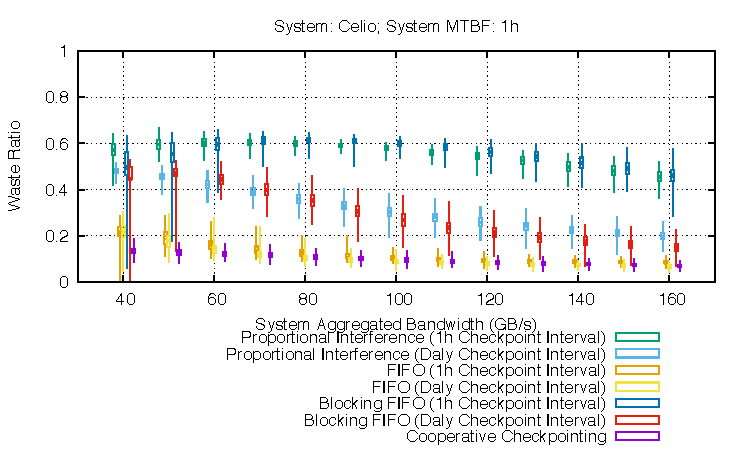
\includegraphics[width=\linewidth]{sim/figures/synthetic-01hMTBF-waste-celio.pdf}
  \end{center}
  \caption{Waste ratio as a function of the system bandwidth for the
    seven I/O and Checkpointing scheduling strategies, and the Cielo
    workload \label{fig:cielo-1hmtbf}}
\end{figure}

First, we explore the performance of each approach under heavy risks
of failures. Figure~\ref{fig:cielo-1hmtbf} represents the waste ratio
on Cielo, assuming the MTBF of the system was 1h. We vary the
filesystem bandwidth from 40 GB/s to 160GB/s in order to evaluate the
impact of this parameter. We observe 3 classes of behavior: \propfixed
and \bfifofixed exhibit a waste ratio that decrease as the bandwidth
increases, but remains above 40\% even with a high available
bandwidth; \fifodaly, \fifofixed, and \cooperative quickly decrese at
only 20\% of waste or less, and reach the theoretical model
performance; and \propdaly and \bfifodaly start at the same level of
efficiency as \propfixed and \bfifofixed, and reach the 20\% of waste
as the bandwidth increases.

This figure shows that with a high frequency of failures, providing
each application with the appropriate checkpoint interval is central
to relieve the filesystem from unecessary (or even detrimental)
checkpoints, but this is not the sole criteria that should be taken
into account. The two strategies that remain with a high waste despite
a high bandwidth rely on a fixed 1h interval. As the figure
illustrates, simply relying on the Daly checkpointing period is not
sufficient to reach the best performance under constrained bandwidth:
at 60GB/s for the filesystem, \propdaly and \bfifodaly experience
twice the waste of the other strategies relying on the same value for
the checkpointing period. All strategies that decouple the execution
of the application from the filesystem availability (\fifodaly,
\fifofixed, \cooperative) exhibit much better performance despite low
bandwidth.

Notably, \cooperative remains the most efficient technique under all
conditions, and reaches the theoretical performance given by
Equation~\eqref{eq.totalwaste} in the case of a stead state
analysis. This illustrates the efficiency of the proposed heuristic
(Equations~\eqref{eq.heuristicpart1} and~\eqref{eq.heuristicpart2}) to
schedule checkpoints and I/O in a way that avoids interferences,
allowing the system to behave as if no interference was experienced,
in most cases. The high variation shows that a minority of the runs
experienced a significantly higher waste.

\begin{figure}
  \begin{center}
    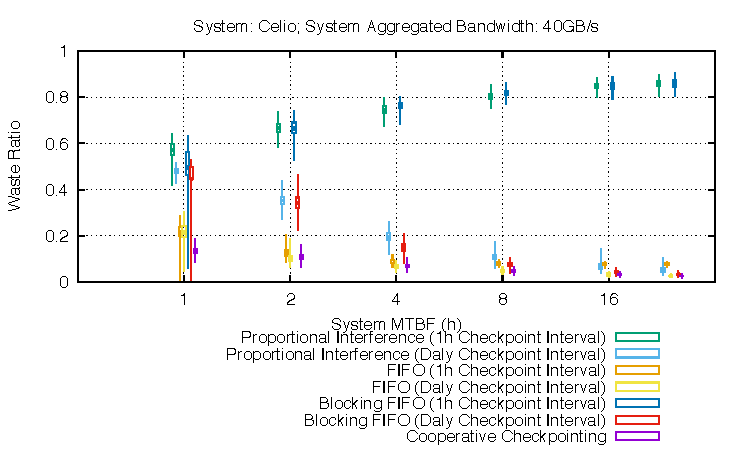
\includegraphics[width=\linewidth]{sim/figures/synthetic-040gbs-waste-celio.pdf}
  \end{center}
  \caption{Waste ratio as a function of the system MTBF for the
    seven I/O and Checkpointing scheduling strategies, and the Cielo
    workload \label{fig:cielo-40gbs}}
\end{figure}

Second, we explore the performance of each approach under low
bandwidth (and thus high risk of
interference). Figure~\ref{fig:cielo-40gbs} represents the waste ratio
on Cielo, assuming the aggregated filesystem bandwidth of the system
was 40GB/s. We vary the system MTBF from 1h (2 years of node MTBF) to
24h (48 years of node MTBF) in order to evaluate the impact of this
parameter. Similarly to Figure~\ref{fig:cielo-1hmtbf}, we observe 3
classes of behavior: \propfixed and \bfifofixed exhibit a waste ratio
that remains constant around 80\% for all values of the MTBF. These
appraoch are critically dependent on the filesystem bandwidth, and a
lower frequency of failures does not significantly improve their
performance. The I/O subsystem is saturated, and the applications
spends most of their time waiting for it. \fifodaly, \fifofixed, and
\cooperative quickly fall at only 20\% of waste or less, and reach
the theoretical model performance; and \propdaly and \bfifodaly start
at the same level of efficiency as \propfixed and \bfifofixed, and
reach the 20\% of waste as the bandwidth increases.

For all the strategies that integrate the Daly checkpointing period
optimization, increasing the MTBF reduces the amount of I/O required
and thus enables to manage a constrained bandwidth easily. All
strategies that schedule the bandwidth are succesful at increasing the
efficiency to values very close to the theoretical model. More
suprisingly, the simple FIFO scheduling of checkpoints with fixed
chekpoint interval (\bfifofixed) is capable of reaching a performance
comparable to the one of the strategies that reduce the number of
checkpoints. This is due to the significant reduction in interference
due to the reduction of number of restarts with an MTBF of 8h. As soon
as the number of restarting applications decreases, the filesystem
sollicitation decreases sufficiently to avoid long delays in non blocking
approaches, as is illustrated by the performance of \fifofixed at 2h
of MTBF.

\subsection{Prospective Systems}


% !TEX root =  ipdps18.tex

\section{Related Works}\label{sec:related}
% Primary: Kurt

We survey related work in this section. We first discuss papers related to I/O
pressure due to checkpointing, followed by those related to avoiding I/O
interference.  We note that these techniques are not necessarily independent;
reducing I/O pressure will generally reduce the likelihood of interference.
Therefore, we attempt to limit our I/O interference discussion to those
techniques which consider the global scheduling of checkpoints and/or general
I/O across a platform.

%\todo[inline]{kbf: I am unsure about this breakdown.  These two things do not
%seem independent; reducing pressure seems to al reduce interference ...}

\subsection{Checkpointing and I/O}

For a single application, the optimal checkpointing period is given by the
Young/Daly formula~\cite{young74,daly04}. This period minimizes the platform
waste, defined as the fraction of the execution time that does not contribute
to the progress of the application (the time \emph{wasted}).  There are two
sources of waste, the time spent taking checkpoints (which calls for longer
checkpoint periods), and the time needed to recover and re-execute after each
failure (which calls for shorter checkpoint periods), The Young/Daly period
achieves the optimal trade-off between both sources to minimize the total
waste.  However, this optimal period may put too much pressure on the I/O
system. It is possible to use a longer, sub-optimal, period that would incur
less pressure and still lead to a reasonable waste. S. Arunagiri et
al.~\cite{Arunagiri2009} have studied such trade-offs and they have shown, both
analytically and instantiating the model with four real-life platforms, that a
great decrease in I/O requirement can be achieved  at the price of a small
increase of the waste.

\subsection{Reducing I/O Pressure}

Optimizations that target reducing I/O pressure from a single application can
generally be divided into two classes; those that attempt to hide or reduce the
checkpoint commit times without reducing the volume of data, and those that
reduce commit times by reducing checkpoint volumes. 

Strategies that attempt to hide checkpoint times include
Diskless~\cite{Plank98Diskless} and remote checkpoint
protocols~\cite{Cornwell11RemoteBLCR,Stellner96CoCheck,Zandy99ProcessHijacking}
which leverage the typically higher available bandwidths to the network or
other storage media like RAM in order to mitigate the performance of slower
storage media like spinning or solid-state disks. Additionally, remotely stored
checkpoints have the additional benefit of allowing systems to survive
non-transient node failures. Similarly, multi-level checkpoint protocols like
SCR~\cite{Moody10SCR,Vaidya95TwoLevel} attempt to hide checkpoint commit times
by writing checkpoints to RAM, flash storage, or local disk on the compute
nodes~\cite{Kougkas2016} in addition to the parallel file system thereby
improving checkpoint or general I/O bandwidth.  Finally, checkpoint-specific
file systems like PLFS~\cite{Bent09PLFS} leverage the I/O patterns and
characteristics specific to checkpoint data to optimize checkpoint data
transfers to/from parallel file systems and therefore reduce checkpoint commit
times.

Those strategies which attempt to reduce checkpoint sizes includes \emph{memory
exclusion} which leverage user-directives or other hints to exclude portions of
process address spaces from checkpoints~\cite{Plank99MemoryExclusion}.
Additionally, incremental checkpointing protocols reduce checkpoint volumes by
utilizing the OS's memory page protection facilities to detect and save only
pages that have been updated between consecutive
checkpoints~\cite{Bronevetsky09Compiler,
Chen97CLIP,Elnozahy92ConsistentCheckpointing,Li94ConcurrentCheckpointing,
Plank94Libckpt,Paun10IncrementalWeibull,Kiswany08stdchk}.  Similarly, page-based
hashing techniques can also be used to avoid checkpointing pages that have been
written to but whose content has not changed~\cite{Ferreira11Libhashckpt}.
Finally, compression-based techniques use standard compression algorithms to
reduce checkpoint volumes.  Li and Fuchs implemented a compiler-based
checkpointing approach, which exploited compile time information to compress
checkpoints~\cite{Li90CATCH}.  Plank and Li proposed in-memory checkpoint
compression~\cite{Plank94ICKP}, and related, Plank et al. proposed
\textit{differential compression} to reduce checkpoint sizes for incremental
checkpoints~\cite{Plank95CompressedDiff}.  Tanzima et al. have shown that
similarities amongst checkpoint data from different processes can be exploited
to compress and reduce checkpoint data volumes~\cite{tanzima12mcrengine}.
Sasaki   et   al  proposed   a   lossy
compression method based on wavelet transform
and  vector  quantization and   applied  their  compression
method  to   checkpoints of a   production   climate  application~\cite{sasaki2015}.

 \subsection{Avoiding I/O interference}

Most closely related to our work, a number of studies have considered the
global scheduling of checkpoints and other I/O across the platform to reduce
the overall congestion therefore increase performance.  Aupy et
al.~\cite{Aupy:2017:Periodic} presented a decentralized I/O scheduling
technique for minimizing the congestion due to checkpoint interference by
taking advantage of the observed periodic and deterministic nature of HPC
application checkpoints and I/O.  This technique allows the job scheduler to
pre-define each application’s I/O behavior for their entire execution.
Similarly, a number of works have investigated the efficiency of online
schedulers for data intensive~\cite{Groot2013,Sim:2015:AnalyzeThis} and HPC
workload
I/O~\cite{Dorier2014,Gainaru:2015:Scheduling,Zhou:2015:IOAware,Herbein2016}.
Finally, a number of works have investigated utilizing system reliability
information recorded on the system~\cite{Oliner:2006:Cooperative} and the
statistical properties of these failures~\cite{Tiwari:2014:Lazy} to determine
effective checkpoint intervals for the portion of the system used by the
workload.

\subsection{Summary}

This present work distinguishes itself from these previous studies in a number
of important ways.  First, this technique is agnostic to the I/O patterns of
the considered applications and does not require deterministic I/O behavior.
Also, this technique attempts to optimize the efficiency of the entire
platform, with the changing workloads and failures running on that platform,
rather than just considering one workload. In addition, this approach can be
used in environments where I/O is highly constrained and Daly/Young's formula
is not appropriate.  Finally, \todo[inline]{kbf: Add more here on novelty ...}

\section{Concluding Remarks}
\label{sec:conclusion}

In this paper we presented a comprehensive model to capture interference
between multiple applications performing fault-tolerance related I/O
on a shared HPC system. We proved that ... We designed multiple algorithms
to schedule and order the checkpointing I/O workload, with the intent of
diminishing the average slowdown sustained by applications on the
platform induced by sharing the I/O subsystem, \ie improve the throughput
of the platform. We designed a event-based simulator that permits
executing typical HPC workloads on current and prospective systems.
With this simulator we have been able to offer guidances as to the
prefered heuristics for scheduling checkpoint workloads, and the
general I/O requirements for future HPC systems to sustain checkpointing.

\section*{Acknowledgement}

This material is based in part upon work supported by the National
Science Foundation under Grant Number 1564133, ``Toward Extreme Scale
Fault-Tolerance: Exploration Methods, Comparative Studies and Decision
Processes''.

\bibliographystyle{IEEEtran}
\bibliography{biblio}

%
%%%%%%%%%%%%%%%%%%%%%%%%%%%%%%%%%%%%%%%%%%%%%%%%%%%%%%%%%%%%%%%%%%%%%%%%
% FOLLOWUP TEXT IS OLDER AND MAY NEED MERGING OR DISCARDING
%%%%%%%%%%%%%%%%%%%%%%%%%%%%%%%%%%%%%%%%%%%%%%%%%%%%%%%%%%%%%%%%%%%%%%%%

\newpage
\appendix

\section{Older text}





\section{Optimal Cooperative Checkpointing Strategy}
\label{sec.strategy}

\subsection{With Burst Buffers}

We slightly change the machine model, and will consider that, in addition
to the global PFS, each node is provisioned with a local stage-in I/O
burst buffer. With burst buffers, $\ckpt{i}$ still represents the time it
takes to upload the checkpoint to the stable storage (the file system).
However, the availability of burst buffers permits a reduction in the
apparent time for the checkpoints as experienced by application idle
time. Note that under I/O constraints on the PFS, checkpoints may remain
in burst buffers (which is not a stable storage) until sufficient
PFS bandwidth is available.

Consider Algorithm~\ref{alg.withbb}: every $\period{i}$ time
units, each application of class $\app{i}$ takes a checkpoint and save
it onto the next free slot on the burst buffer; a global shared FIFO
queue transfers checkpoints from active slots in burst buffers onto
the parallel file system following the FIFO queue order.

\algblockdefx{Process}{EndProcess}[1]{\textbf{On Process} #1}{\textbf{End Process}}
\algnotext{EndProcess}
\algblockdefx{Every}{DoneEvery}[1]{\textbf{Every } #1}{\textbf{Done}}
\algnotext{DoneEvery}
\algblockdefx{When}{DoneWhen}[1]{\textbf{When } #1}{\textbf{Done}}
\algnotext{DoneWhen}
\algloopdefx{If}[1]{\textbf{If} #1 \textbf{then}}
\begin{algorithm}
\caption{Cooperative Checkpointing Algorithm with Burst Buffers}
\label{alg.withbb}
\begin{algorithmic}
\State \textbf{var} $transfer\_queue$, a FIFO initially empty
\Process{$p$, belonging to application $\application{i}{j}$ of class $\app{i}$}
   \State \textbf{var} $slots$ set of burst buffer files that can
   store a checkpoint
   \Every{$\period{i}$ time units}
           \State $slot  \gets $ oldest slot that is not being used for transfer
           \State Checkpoint application state into $slot$
           \If{$slot$ is marked done transferring}
                  \State Append $(p, slot)$ to $transfer\_queue$
    \DoneEvery
\EndProcess

\Process{$T$}
   \When{$transfer\_queue$ is not empty}
       \State Pop $slot$ from $transfer\_queue$
       \State Mark $slot$ as being transferred
       \State Transfer Checkpoint in $slot$ to File System
       \State Mark $slot$ as done transferring
   \DoneWhen
\EndProcess
\end{algorithmic}
\end{algorithm}

\begin{theorem}
  Algorithm~\ref{alg.withbb} ensures that all applications of class $\app{i}$
  checkpoint at most every $max(\sum_j\nbapp{j}*\ckpt{j}, \period{i})$
  time units, and requires only a burst buffer capable of storing 2
  checkpoints per process.
\end{theorem}

\begin{proof}
  \todo{This derives from $\sum_i \frac{\ckpt{i}}{\period{i}} \leq 1$,
    but should be done properly.}
\end{proof}

The theorem does provide a lower bound for the platform waste.\todo[inline]{the 2 storages holds only after the optimization, doesn't it? Or is it also a consequence of the above "proof" sketch?}
However, we have a FIFO system, and some applications may incur
a re-execution time larger than $P_{i}$. What is the worst case?
A first optimization is the following: when a checkpoint is taken
    by a given application, we check whether its previous checkpoint is
    still in the queue from the burst buffer to the file system. If yes, the new
checkpoint should \emph{replace} the old one, keeping the same position in the queue.
With this optimization, there is at most two checkpoints per application in the queue,
one being currently transferred and one waiting.
Then the worst case is to wait for the checkpoint of all the other applications.
Formally, the maximal re-execution time for application
$\application{i}{j}$ of class
$\app{i}$ is
$$\max(P_{i}, \sum_{k=1}^{\nbapps} n_{k}C_{k} - C_{i})$$

 \todo[inline]{Discussed at JLESC meeting: size of burst buffer can be
    bounded by 2 checkpoints easily, and it should be: if there are 3
    checkpoints in the burst buffer, then the first one might be being
    transferred, but this means that the 2nd is useless as we already
    reached the 3rd one. The 2nd should be discarded and its slot in
    the FIFO queue should be taken by the 3rd.}

  \todo[inline]{No clear what qualifies for burst buffers here, but
    currently the NVM bandwidth is (1) significantly lower than the
    network bandwidth, and (2) unidirectional. This might change in
    the future, but at least today it seems cheaper to use a
    buddy-checkpointing approach.}%


\subsection{Without Burst Buffers}

Without a local caching mechanism\footnote{Note that this case covers ``shared'' burst-buffers, where the
PFS contains an intermediate stage-in area (presumably with SSD drives, a much higher bandwidth, and possibly contention reduced to a subset of the nodes it serves, but provides for stable/persistent storage as soon as the data is committed to the shared burst-buffer.}, the times at which to take the checkpoint
must be scheduled to avoid any kind of checkpoint-checkpoint
interference (which can only waste resources, as all interfering
applications are slowed down while blocking on non-productive
operations). We consider here a centralized scheduler that decides at
any time what next application should checkpoint, and when.

The scheduler remembers when each application $\application{i}{j}$ of class
$\app{i}$ last initiated a checkpoint. We then define $\lastckpt{i}{j}$
as the time since the last checkpoint $\application{i}{j}$ started
(or since the start of $\application{i}{j}$ if none has been taken yet).
As soon as $\application{i}{j}$ has executed for $P_{i}$ time-units,
it is put in the checkpointing pool $\pool$ by the centralized scheduler. It
continues executing until it is selected from the pool to checkpoint.

Which application in the pool should be selected to checkpoint?
Assume that some previous checkpoint terminates at time $t$,
and let
$$\pool = \{ \application{i_{1}}{j_{1}}, \dots, \application{i_{k}}{j_{k}} \}$$
be the set of applications  in the pool at time $t$. All these applications are
candidate to checkpointing. At time $t$, each application $\application{i_{\ell}}{j_{\ell}} \in \pool$
has been executing for  $\lastckpt{i_{\ell}}{j_{\ell}}$ time-units.

If we select $\application{i_{\ell}}{j_{\ell}}$ to checkpoint (in time $C_{j_{\ell}}$),
and if there is a failure during that checkpoint, the time lost by every other application
$\application{i_{m}}{j_{m}} \in \pool$, $m \neq \ell$, is (in expectation) equal to
 $\lastckpt{i_m}{j_m} + \frac{C_{j_{\ell}}}{2}$.
We define the risk incurred by application
$\application{i_{m}}{j_{m}} \in \pool$, $m \neq \ell$
as its potential waste, which is the time lost divided by its MTBF $\frac{\mtbfplat}{\nbnodes{i}}$,
times the number $\nbnodes{i_m}$ processors enrolled by this application, i.e.
$$ \frac{\nbnodes{i_{m}}}{\mtbfplat}  (\lastckpt{i_m}{j_m} + \frac{C_{j_{\ell}}}{2})
\times \nbnodes{i_m} $$
Altogether, selecting $\application{i_{\ell}}{j_{\ell}}$ to checkpoint leads to a total risk
$$\risk(\application{i_{\ell}}{j_{\ell}}) = \sum_{1 \leq m \leq k, m \neq \ell} \frac{\nbnodes{i_{m}}^{2}}{\mtbfplat}  \times (\lastckpt{i_m}{j_m} + \frac{C_{j_{\ell}}}{2})$$
  for all applications that stayed in the pool.

We greedily choose the application in the pool that minimizes the risk:
$$\application{i_{\ell}}{j_{\ell}} = Argmin_{\application{i_m}{j_m} \in \pool} \risk(\application{i_m}{j_m})$$

%At the end of each checkpointing, the scheduler selects
%$\application{i}{j}$ such that
%$$
%\left\{
%\begin{array}{l}
%\nbnodes{i}(\frac{\wastefct{i}{\lastckpt{i}{j}}}{\wastefct{i}{\period{i}}}) \textrm{ if }\lastckpt{i}{j}\geq\period{i}\\
%0\textrm{ if }\lastckpt{i}{j}<\period{i}\\
%\end{array}\right.$$
%is maximal and strictly superior to 0.

Two remarks:
\begin{itemize}
\item Because we put applications in the pool only after they have run for $P_{i}$ times-steps,
this greedy algorithm guarantees Young/Daly periods to every application
whenever there is non conflict to access I/O resources.
\item The final schedule is not periodic. Instead, it is constructed dynamically
after each checkpoint completion. Computing the actual waste can be achieved
through simulation, and compared to the lower bound of Section~\ref{sec.optimal}.
\end{itemize}


\end{document}
